%
% ---------- header -----------------------------------------------------------
%
% project       kaneton
%
% license       kaneton
%
% file          /home/mycure/kaneton/view/exam/mips/2007/final/final.tex
%
% created       julien quintard   [mon may 14 21:49:31 2007]
% updated       julien quintard   [thu may 22 19:46:52 2008]
%

%
% ---------- setup ------------------------------------------------------------
%

%
% path
%

\def\path{../../../..}

%
% template
%

%%
%% licence       kaneton licence
%%
%% project       kaneton
%%
%% file          /home/mycure/kaneton/view/templates/exam.tex
%%
%% created       julien quintard   [fri dec  2 22:20:57 2005]
%% updated       julien quintard   [mon feb 20 23:01:50 2006]
%%

%
% compile mode
%

%
% ---------- header -----------------------------------------------------------
%
% project       kaneton
%
% license       kaneton
%
% file          /home/mycure/kane...w/talk/presentations/kaneton/kaneton.tex
%
% created       julien quintard   [mon may 14 21:02:29 2007]
% updated       julien quintard   [sun feb  6 20:50:37 2011]
%

%
% ---------- setup ------------------------------------------------------------
%

%
% path
%

\def\path{../../..}

%
% template
%

%
% ---------- header -----------------------------------------------------------
%
% project       kaneton
%
% license       kaneton
%
% file          /home/mycure/kaneton/view/template/talk.tex
%
% created       julien quintard   [wed may 16 18:17:37 2007]
% updated       julien quintard   [fri may 23 19:28:10 2008]
%

%
% ---------- class ------------------------------------------------------------
%

\documentclass[8pt]{beamer}

%
% ---------- common -----------------------------------------------------------
%

\input{\path/package/opk/presentation.tex}


%
% title
%

\title{kaneton}

%
% document
%

\begin{document}

%
% title frame
%

\begin{frame}
  \titlepage
\end{frame}

%
% outline frame
%

\begin{frame}
  \frametitle{Outline}

  \tableofcontents
\end{frame}

%
% ---------- text -------------------------------------------------------------
%


%
% overview
%

\section{Overview}

% 1)

\begin{frame}
  \frametitle{Introduction}

  \term{kaneton} is an educational project intended for students to undertake
  in order to learn about operating system internals.
\end{frame}

% 2)

\begin{frame}
  \frametitle{History}

  \begin{itemize}
    \item[2004]
      \name{Julien Quintard} and \name{Jean-Pascal Billaud} decide
      to introduce an optional low-level programming course to first-year
      enginnering students, now known as \name{kastor};
    \item[2004]
      The course having been well received, \name{SRS - Syst\`emes, R\'eseaux,
      S\'ecurit\'e} students ask them to give such an introductory course the
      same year.
    \item[2005]
      The authorization is given to them to teach a kernel development course
      to \name{SRS} students, from January to October. They therefore decide
      to provide students with the design of a microkernel and let the students
      develop it from scratch, their way. \name{kaneton} is born.
    \item[2006]
      After \name{Jean-Pascal Billaud} fled to \name{VMWare}, \name{Julien
      Quintard} started developing a reference implementation and gave
      students this year a skeleton they had to complete. In addition,
      \name{Cedric Aubouy} and \name{Renaud Lienhart} joined the teaching
      team this year.

      \-

      Besides, the \name{LSE - Laboratoire Syst\`eme EPITA} joined the project
      by putting two students on the development of the \name{kaneton}
      research implementation. \name{Matthieu Bucchianeri} and \name{Renaud
      Voltz} thus joined the project.
  \end{itemize}
\end{frame}


% 3)

\begin{frame}
  \frametitle{History}

  \begin{itemize}
    \item[2007]
      This year, \name{Matthieu Bucchianeri} and \name{Renaud Voltz} took
      over the project for a year by lecturing the course and managing the
      project.

      \-

      \name{Julian Pidancet} and \name{Pierre Duteil} joined the project
      as part of the \name{LSE} but \name{Pierre Duteil} had to leave the
      project. Therefore, \name{Elie Bleton}, who was working at the
      \name{LRDE} before, joined the project.
    \item[2008]
      \name{Julian Pidancet} and \name{Elie Bleton} took over this year
      while \name{Laurent Lec} and \name{Nicolas Grandemange} joined as part
      of the \name{LSE}.

      \-

      At the end of this year, after problems with some students as well as
      conflicts with the \name{LSE}, \name{kaneton} maintainers decided not
      to work with the laboratory anymore.
    \item[2009]
      \name{EPITA} alumni were contacted and joined the educational project
      including \name{Francois Goudal}, \name{Benoit Marcot},
      \name{Enguerrand Raymond}, \name{Jean Guyader} but also
      \name{Fabien Le-Mentec}, an \name{EPITECH} alumnus.
  \end{itemize}
\end{frame}

% 4)

\begin{frame}
  \frametitle{Model}

  The project consists for students to fill in some missing parts of the
  kernel.

  \-

  However, note that, unlike \name{Tiger}, the missing parts will never
  be two lines long.

  \-

  Indeed, in \name{kaneton}, students are asked to implement a feature, say,
  providing memory management. Thus, students are free, in a certain way,
  to implement such a feature as they wish.

  \-

  Since the testing usually consists in verifying that the kernel is able
  to provide the functionality, students should be, most of the time, able
  to implement whatever algorithms \etc{} they wish.
\end{frame}

% 5)

\begin{frame}
  \frametitle{People}

  Let's present the people working on the educational project from where they
  studied to what they are now doing:

  \begin{itemize}
    \item
      \name{Francois Goudal};
    \item
      \name{Benoit Marcot};
    \item
      \name{Jean Guyader};
    \item
      \name{Baptiste Afsa}
    \item
      \name{Louis Vatier}; and
    \item
      \name{Julien Quintard}.
  \end{itemize}
\end{frame}

% 6)

\begin{frame}
  \frametitle{Project}

  \name{kaneton} is an important assignment of the \name{SRS}/\name{GISTR}
  curriculum and, as such, must be taken seriously.

  \-

  Especially, in the last years, \name{EPITA} decided to reduce the duration
  of the project to \term{three} months.

  \-

  As such, the other assignments imposed by the specializations in this
  period have been reduced so that students can focus on \name{kaneton}.
\end{frame}

%
% design
%

\section{Design}

% 1)

\begin{frame}
  \frametitle{Overview}

  The kaneton kernel is very different from the kernels you might be
  familiar with, especially the well-known \name{Windows}, \name{Linux},
  \name{BSD} and so forth.
\end{frame}

% 2)

\begin{frame}
  \frametitle{Microkernel}

  First, kaneton is a microkernel, making it modular from the design
  perspective as well as providing properties such as security.
\end{frame}

% 3)

\begin{frame}
  \frametitle{Distributed Computing}

  kaneton has been designed from the ground up for providing the operarting
  system advanced distributed computing features.
\end{frame}

% 4)

\begin{frame}
  \frametitle{Portability}

  kaneton has been designed with portability in mind, especially through
  a specific portability system that perfectly fits the kernel design.
\end{frame}

% 5)

\begin{frame}
  \frametitle{Organisation}

  Besides being a microkernel, kaneton is well organised in the inside,
  splitting functionalites into objects and managers.
\end{frame}

%
% stages
%

\section{Stages}

% 1)

\begin{frame}
  \frametitle{k0}

  The first project, named \term{k0}, consists for students to learn
  about low-level programming.

  \-

  This project comes with a lecture regarding the boot system as well
  as a practical session.

  \-

  \name{Francois Goudal} will be in charge of this stage which will last for
  a week.
\end{frame}

% 2)

\begin{frame}
  \frametitle{k1}

  \term{k1} consists for students to provide the kaneton microkernel the
  capacity to handle events.

  \-

  During this stage, a lecture on general kernel principles and a lecture on
  interrupts will be taught.

  \-

  \name{Julien Quintard} will be in charge of this stage which will last
  for a single week.

  \-

  Note that, starting with \name{k1}, the student snapshot will be used which
  provide students a development environment, making kernel development easier.
\end{frame}

% 3)

\begin{frame}
  \frametitle{k2}

  \term{k2} consists for students to provide the kaneton microkernel a
  memory management unit so that applications as well as the kernel itself
  can reserve, share \etc{} memory.

  \-

  During this stage, a lecture on portability as well as lectures on
  memory management will be taught.

  \-

  \name{Francois Goudal} will be in charge of this stage which will last
  for three weeks.
\end{frame}

% 4)

\begin{frame}
  \frametitle{k3}

  In \term{k3}, students will have to provide kaneton with execution contexts
  such that the kernel can execute multiple threads at the \textit{same} time.

  \-

  Lectures, during this stage, will discuss topics such as interrupts,
  concurrency, multi-processing, scheduling \etc{}

  \-

  \name{Benoit Marcot} will be in charge of this stage which will last for
  three weeks.
\end{frame}

% 5)

\begin{frame}
  \frametitle{Evaluation}

  For every stage, students will have the possibility to test their
  implementation by running, a limited number of times, the test suite used
  for evaluating their work.

  \-

  Besides, at the end of each stage, after submission, the kaneton test system
  will run the test suite and issue a mark according to the test results.

  \-

  Additionally, an exam will take place at the end of the semester to make
  sure that the notions tackled throughout the course are well understood
  by every student.
\end{frame}

%
% tools
%

\section{Tools}

% 1)

\begin{frame}
  \frametitle{Overview}

  The kaneton educational project relies on tools, sometimes developed
  internally.
\end{frame}

% 2)

\begin{frame}
  \frametitle{Web Site}

  The web site contains the documentation including design papers,
  the assignments \etc{} but also hosts the wiki which should be
  the starting point for every student seeking information.

  \-

  Noteworthy is that the wiki contains courses regarding the
  inline assembly, linking, pre-processing and so on. Students
  are invited to read them all as they will come handy when
  developing the kaneton stages.

  \-

  \name{Julien Quintard} should be contacted for requests regarding the
  web site and wiki.
\end{frame}

% 3)

\begin{frame}
  \frametitle{Snapshot}

  The student snapshot has been automatically generated from the current
  kaneton implementation.

  \-

  \name{Francois Goudal} is in charge of this process, hence should be
  contacted if you believe there is a mistake.
\end{frame}

% 4)

\begin{frame}
  \frametitle{Cheat}

  Every student's kaneton implementation will be tested to make sure that
  students did not cheat by relying on implementations by previous or
  current students.

  \-

  \name{Julien Quintard} is in charge of this tool.
\end{frame}

% 5)

\begin{frame}
  \frametitle{Test}

  Students' implementation will be tested in a real environment by applying
  a complete test suite; hence, validating the implementation's behaviour.

  \-

  \name{Jean Guyader} is responsible of this tool and should be contacted
  if necessary.
\end{frame}

%
% information
%

\section{Information}

% 1)

\begin{frame}
  \frametitle{Support}

  \begin{enumerate}
    \item
      \term{Website}

      \-

      You will find on \location{http://kaneton.opaak.org} documents regarding
      the project from the design to the implementation;
    \item
      \term{Wiki}

      \-

      The wiki \location{http://wiki.opaak.org} is the best way to get
      technical information as well as to help other students by adding
      and/or improving pages' contents;
    \item
      \term{Mailing-List}

      \-

      The kaneton educational students mailing-list
      \location{students@kaneton.opaak.org} will be used by teachers as
      an official means for communicating with students.

      \-

      Therefore, every student should subscribe to this mailing-list by sending
      an email to \location{students+subscribe@kaneton.opaak.org}.

      \-

      It is not allowed to post code on the mailing list, or give pointers to
      code in the snapshot that would provide obvious solution to somebody's
      question.
  \end{enumerate}
\end{frame}

% 2)

\begin{frame}
  \frametitle{Groups}

  Except for \name{k0} which is an individual project, the other projects
  from \name{k1} to \name{k3} are done in groups of \term{two} students.

  \-

  Every group is expected to send an email to
  \location{admin@opaak.org}.

  \-

  Note that we will use students' \name{EPITA} email addresses. As such,
  make sure that you check this email box.
\end{frame}

% 3)

\begin{frame}
  \frametitle{Reliance}

  As for \name{Tiger}, every stage depends on the previous one, except
  for \name{k0}.

  \-

  As such, test suites from the previous stages will also be used for both
  testing and marking.

  \-

  Students should therefore make sure to use their test permissions for making
  sure to fix the bugs of previous stages so that such bugs do not impact
  on the current stage results, hence mark.
\end{frame}

% 4)

\begin{frame}
  \frametitle{Machine}

  This year, the machine used by the kaneton educational project will consists
  of the \term{IBM-PC} platform coupled with the \term{IA-32} microprocessor
  architecture \ie{} the most common hardware system on the market.

  \-

  Although it is always best to test your implementation on a real machine,
  it takes time to reboot a real computer. You should therefore use an
  emulator such a \name{QEMU} or \name{Bochs} as they will enable you to
  test your kernel very quickly but they will also let you develop on
  a non-\name{IBM-PC}/\name{IA-32} machine such as a \name{Mac} for example.
\end{frame}

%
% conclusion
%

\section{Conclusion}

% 1)

\begin{frame}
  \frametitle{Concepts}

  Throughout the project, you will learn so many things from terminology,
  to how a computer boots, how the kernel controls the hardware and how it
  provides abstractions as basic as execution contexts.

  \-

  At the end of the project, you will definitely know that nothing is magic
  but purely logic and often actually very simple.
\end{frame}

% 2)

\begin{frame}
  \frametitle{Implementation}

  Although, starting the project by learning how to make a computer execute
  your code, you will end up, after three months, with a running kernel
  and operating system capable of executing programs, the whole on real
  hardware like the machine you have at home.
\end{frame}

% 3)

\begin{frame}
  \frametitle{Changes}

  Over the years, the project has greatly evolved, from a no-implementation
  project, to a reference-based project.

  \-

  However, being a project developed by volunteers willing to dedicate some
  time so that other students can learn, many things are missing and/or
  can be improved including the lectures but also the project implementation.

  \-

  In conclusion, keep in mind that the project exists only because of people
  willing to transfer their knowledge and please respect their effort.
\end{frame}

% 4)

\begin{frame}
  \frametitle{Fun}

  But most of all, kaneton should be about learning through fun!
\end{frame}

% 5)

\begin{frame}
  \frametitle{Reminder}

  Remember to perform the following tasks:

  \begin{itemize}
    \item
      Send an email to \location{admin@opaak.org} regarding the composition
      of your group, before \textbf{Wednesday 16th 2pm} or you will be put
      in a group by force;
    \item
      Subscribe to the students mailing-list
      \location{students@kaneton.opaak.org} by sending an email to
      \location{students+subscribe@kaneton.opaak.org};
    \item
      Watch closely the \name{Wiki} at \location{http://wiki.opaak.org} by
      subscribing the \name{RSS} feed for example;
    \item
      We advise SRS/GISTR lab roots to set up a \name{Xen}-based environment
      as testing on emulators only will become difficult over time;
    \item
      Students must have a ``rack'' containing a \name{POSIX}-compilant
      operating system for the \name{k0} practical session.
  \end{itemize}
\end{frame}

\end{document}


%
% class
%

\documentclass[10pt,a4wide]{article}

%
% packages
%

\usepackage[english]{babel}
\usepackage[T1]{fontenc}
\usepackage{a4wide}
\usepackage{graphicx}
\usepackage{fancyheadings}
\usepackage{multicol}
\usepackage{indentfirst}
\usepackage{color}
\usepackage{ifthen}
\usepackage{comment}
\usepackage{verbatim}
\usepackage{aeguill}

\pagestyle{fancy}

\setlength{\footrulewidth}{0.3pt}
\setlength{\parindent}{0.3cm}
\setlength{\parskip}{2ex plus 0.5ex minus 0.2ex}

%
% correction environment
%

\newenvironment{correction}%
   {
     \ifthenelse
	 {
	   \equal{\kaneton-latex}{subject}
	 }
	 {
	   \comment
	 }
	 {
	   \textbf{\color{red}{ ----- correction}}
	 }
   }%
   {
     \ifthenelse
	 {
	   \equal{\kaneton-latex}{subject}
	 }
	 {
	   \endcomment
	 }
	 {
	   \textbf{\color{red}{ ----- /correction}}
	 }
   }

%
% header
%

\rfoot{\scriptsize{Exam}}

\date{\scriptsize{\today}}


%
% header
%

\lhead{\scriptsize{2006}}

%
% title
%

\title{Examen d'Architecture MIPS}

%
% authors
%

\author{\small{Julien Quintard}}

%
% document
%

\begin{document}

%
% title
%

\maketitle

%
% indentation
%

\indentation{}

%
% --------- information -------------------------------------------------------
%

\begin{center}

\textbf{Documents Interdits}

\textbf{Dur\'ee 2 heures}

\scriptsize{Une copie bien pr\'esent\'ee avec des sch\'emas propres et
	    lisibles sera toujours mieux not\'ee qu'une autre.}
\end{center}

%
% --------- text --------------------------------------------------------------
%

On consid\`ere la fonction \textbf{villageoise}() suivante qui effectue
l'op\'eration de \textit{Gauss} sur une ligne \textit{j} par rapport \`a
la ligne \textit{k}.

La matrice \textit{m} est une matrice carr\'ee de taille \textit{size}.

On suppose qu'une ligne de la matrice contient 1024 \'el\'ements
et que l'adresse de la matrice est align\'ee sur 4096.

\begin{verbatim}
int*            villageoise(int* m,
                            unsigned int j,
                            unsigned int k,
                            unsigned int size,
                            int e)
{
  int           i;

  for (i = 0; i < size; i++)
    m[(j * size) + i] = m[(j * size) + i] - m[(k * size) + i] * e;

  return (m);
}
\end{verbatim}

Ce code est ensuite compil\'e pour une r\'ealisation \textbf{non pipeline}
du processeur MIPS. Le code assembleur produit est le suivant.

\begin{itemize}
  \item
    \textit{R5} contient l'adresse de la ligne \textit{j}.
  \item
    \textit{R6} contient l'adresse de la ligne \textit{k}.
  \item
    \textit{R7} contient l'adresse de la fin de la ligne \textit{j}.
  \item
    \textit{R8} contient le coefficient \textit{e}.
\end{itemize}

\begin{verbatim}
Loop:    Lw R9, 0(R6)
         Mul R9, R9, R8
         Lw R10, 0(R5)
         Sub R10, R10, R9
         Sw R10, 0(R5)

         Addiu R6, R6, 4
         Addiu R5, R5, 4
         Bne R5, R7, Loop
\end{verbatim}

Le processeur MIPS-10 \'etudi\'e est le suivant:

\begin{center}
  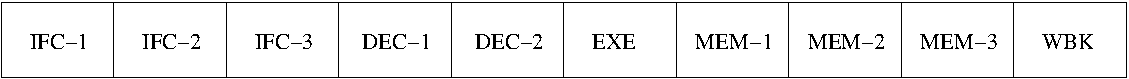
\includegraphics[scale=0.6]{figures/pipeline.pdf}
\end{center}

Comme pour les microprocesseurs profonds \'etudi\'es en cours, les \'etages
\textit{IFC} et \textit{MEM} sont d\'ecoup\'es afin de laisser plus de temps
\`a la m\'emoire pour r\'epondre. Ce MIPS-10 dispose \'egalement d'un
double \'etage \textit{DEC} afin de soulager la complexit\'e de cet \'etage.

Plus pr\'ecis\'ement, l'\'etage \textit{DEC-1} s'occupe de d\'ecoder et
d'extraire les op\'erandes tandis que l'\'etage \textit{DEC-2} se charge,
quant \`a lui, du calcul de l'adresse suivante.

On suppose que ce microprocesseur dispose d'une instruction
\textit{Mul Rd, Rs, Rt} de format R. Dans cette instruction, les 32 bits
de poids faibles du r\'esultat sont rang\'es dans le registre \textit{Rd}.
Pour cette instruction, les 4 \'etages EXE, MEM-1, MEM-2 et MEM-3 sont
remplac\'es par MX-1, MX-2, MX-3 et MX-4.

On supposse que ce microprocesseur dispose d'un cache d'instructions et d'un
cache de donn\'ees. Ces caches sont reli\'es au syst\`eme m\'emoire \`a
travers un Pi-Bus.

On suppose que le cache d'instructions est parfait et ne g\'en\`ere pas de
requ\^etes sur le bus.

Le cache de donn\'ees est un cache \`a correspondance direct de type
\textit{Write Through} et ne dispose pas de buffer d'\'ecriture. Un bloc
de cache comporte 16 octets et le cache a une taille de 4 Koctets.

Lorsque le cache re\c{c}oit une requ\^ete du processeur au cycle \textit{i}
qui n\'ecessite un acc\`es au bus, il \'emet une requ\^ete sur le bus au
cycle \textit{i + 1} et il faut en moyenne 5 cycles pour qu'il obtienne
l'autorisation d'utilisation du bus. Le bus permet de transf\'erer 4 octets
\`a chaque cycle suivant le protocole de Pi-Bus.

En cas de \textit{Miss} sur une lecture, il faut attendre que le bloc soit
enti\`erement lu depuis la m\'emoire, puis, dans le cycle suivant le cache
met \`a jour ses m\'emoires et il faut un cycle suppl\'ementaire pour
r\'epondre au processeur

On suppose que le cache de donn\'ees est vide au d\'ebut de l'ex\'ecution
de la boucle.

%
% fonctionnement
%

\section{Fonctionnement - 2 points}

Modifier le code de la boucle de la fonction \textbf{villageoise}() de telle
mani\`ere qu'il soit ex\'ecutable par le processeur pipeline MIPS 10 \'etages.

\begin{correction}

  Il faut ajouter \textbf{4} \textit{delay slots} apr\`es chaque
  branchement.

  \begin{verbatim}
  Loop:    Lw R9, 0(R6)
           Mul R9, R9, R8
           Lw R10, 0(R5)
           Sub R10, R10, R9
           Sw R10, 0(R5)

           Addiu R6, R6, 4
           Addiu R5, R5, 4
           Bne R5, R7, Loop
           Nop
           Nop
           Nop
           Nop
  \end{verbatim}

\end{correction}

%
% bypasses
%

\section{Bypasses - 4 points}

Veuillez mettre en \'evidence, via une vue simplifi\'ee, les diff\'erents
\textit{bypasses} que comporte ce processeur MIPS-10.

Pour chaque \textit{bypass} vous devrez mettre en place une s\'equence
d'op\'erations mettant en \'evidence l'utilisation d'un tel bypass.

Donner une explication du nombre de \textit{bypasses} trouv\'es par rapport
au MIPS-7 \'etudi\'e en cours. En d'autres termes, ce nombre vous parait
il coh\'erent

\begin{correction}

  \begin{center}
    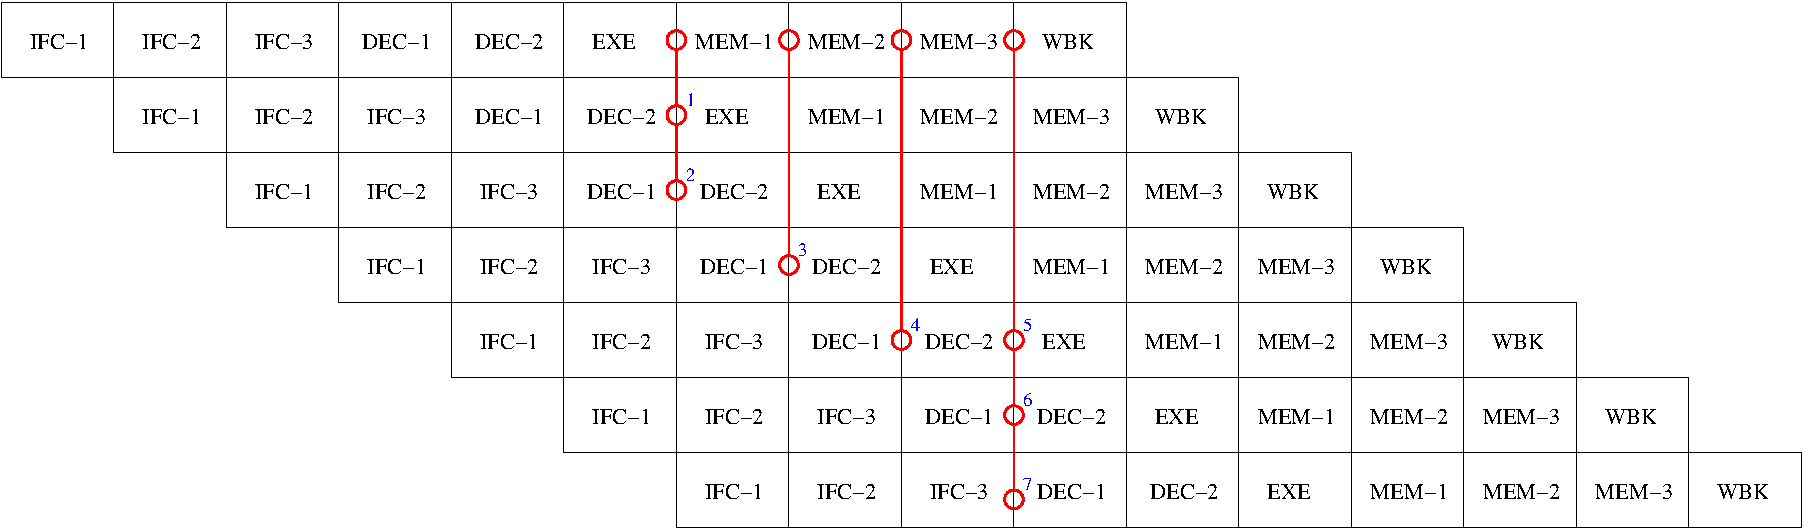
\includegraphics[scale=0.45]{figures/correction-bypasses.pdf}
  \end{center}

  \begin{enumerate}
    \item
      \begin{verbatim}
	Add R3, R2, R1
	Add R5, R4, R3
      \end{verbatim}
    \item
      \begin{verbatim}
	Add R3, R2, R1
	Nop
	Beq R3, R0, Loop
      \end{verbatim}
    \item
      \begin{verbatim}
	Add R3, R2, R1
	Nop
	Nop
	Beq R3, R0, Loop
      \end{verbatim}
    \item
      \begin{verbatim}
	Add R3, R2, R1
	Nop
	Nop
	Nop
	Beq R3, R0, Loop
      \end{verbatim}
    \item
      \begin{verbatim}
	Lw R3, 0(R5)
	Nop
	Nop
	Nop
	Add R5, R4, R3
      \end{verbatim}
    \item
      \begin{verbatim}
	Lw R3, 0(R5)
	Nop
	Nop
	Nop
	Nop
	Beq R3, R0, Loop
      \end{verbatim}
    \item
      \begin{verbatim}
	Lw R3, 0(R5)
	Nop
	Nop
	Nop
	Nop
	Nop
	Beq R3, R0, Loop
      \end{verbatim}
  \end{enumerate}

\end{correction}

%
% analyse simplifiee
%

\section{Analyse Simplifi\'ee - 4 points}

Veuillez d\'ecrire l'ex\'ecution de la boucle de la fonction
\textbf{villageoise}() \`a l'aide d'une vue simplifi\'ee en sp\'ecifiant les
\textit{bypasses} utilis\'es.

Vous devrez ensuite calculer CPI et CPIu.

On consid\`ere que l'on dispose d'un cache de donn\'ees parfait, dans cet
exercice et dans le suivant, afin de mettre les probl\'ematiques d'acc\`es
m\'emoire de c\^ot\'e. Ces probl\'ematiques seront trait\'ees dans le
dernier exercice.

\begin{correction}

  \begin{center}
    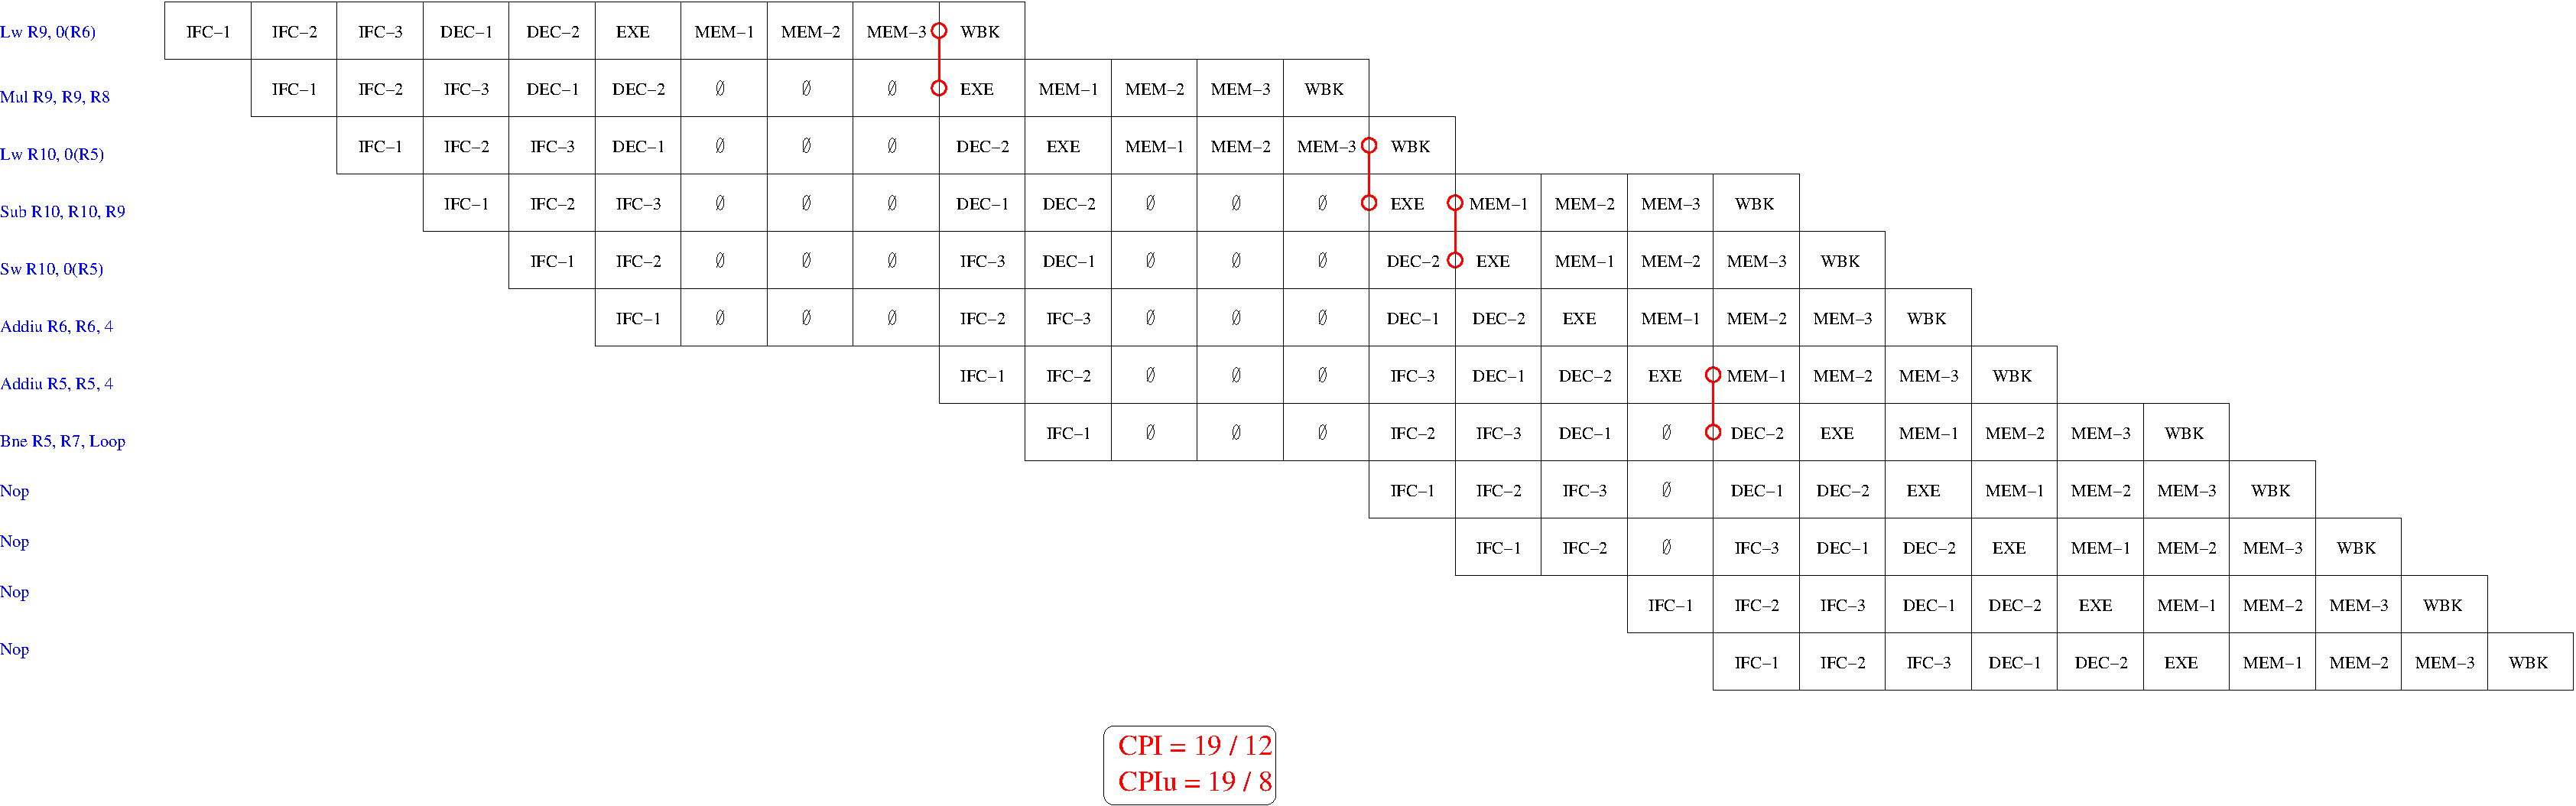
\includegraphics[scale=0.25]{figures/correction-analyse-simplifiee.pdf}
  \end{center}

\end{correction}

%
% optimisation
%

\section{Optimisation - 4 points}

Veuillez appliquer l'optimisation \textit{Software Pipeline} sur
la boucle de la fonction \textbf{villageoise}() de mani\`ere \`a obtenir
les meilleures performances.

Vous \^etes bien entendu autoris\'es \`a effectuer un r\'eordonnancement
afin d'optimiser la boucle obtenue.

Vous calculerez ensuite le CPI et CPIu de cette nouvelle implantation
de la boucle.

Est-ce que l'optimisation \textit{Software Pipeline} est int\'eressante
dans ce cas l\`a? Pourquoi? Quel est le gain ou la perte de performance?

\begin{correction}

  \begin{verbatim}
  Loop:    Sw R11, 0(R5)

           Sub R11, R10, R9

           Lw R9, -8(R6)

           Addiu R5, R5, 4

           Lw R10, -12(R5)

           Bne R5, R7, Loop
           Mul R9, R9, R8
           Nop
           Addiu R6, R6, 4
           Nop
  \end{verbatim}

  CPI = 10 / 10

  CPIu = 10 / 8

\end{correction}

%
% memoire
%

\section{M\'emoire - 6 points}

\textit{Conseil}: Prenez bien en compte toutes les informations
donn\'ees au d\'ebut du document.

Nous consid\'erons dans cette question, l'implantation originale de la
boucle et non son \'evolution \textit{Software Pipeline}.

Veuillez r\'epondre aux questions ci-dessous en justifiant chaque \'el\'ement
intervenant dans vos calculs.

\begin{enumerate}
  \item
    En cas de Miss, combien de cycles sont n\'ecessaires pour une lecture de
    16 octets?

    \begin{correction}

      \begin{verbatim}
	1 +                     ; access
	5 +                     ; bus acquire
	1 +                     ; address
	3 +                     ; address / data
	1 +                     ; data
	1 +                     ; update
	1                       ; response

	= 13 cycles
      \end{verbatim}

    \end{correction}
  \item
    De m\^eme, combien de cycles sont n\'ecessaires pour une \'ecriture de
    4 octets?

    \begin{correction}

      \begin{verbatim}
	1 +                     ; access
	5 +                     ; bus acquire
	1 +                     ; address
	1                       ; data

	= 8 cycles
      \end{verbatim}

    \end{correction}
  \item
    Calculer le nombre moyen de cycles n\'ecessaires au traitement d'un
    \'el\'ement de la matrice.

    Un bon moyen d'effectuer cela pourrait \^etre d'identifier le taux de
    \textit{Miss} dans une boucle et de calculer la p\'enalit\'e
    qu'engendre cette ex\'ecution par rapport \`a une m\'emoire parfaite;
    m\'emoire que nous avons consid\'er\'ee jusqu'ici.

    \begin{correction}

      Une ligne de matrice contient 1024 \'el\'ements soit 4096 octets.
      Une ligne de matrice peut donc \^etre enti\`erement contenue dans le
      cache.

      De ce fait, chaque it\'eration de la boucle va provoquer 2 \textit{Miss},
      un premier pour lire un \'el\'ement de la ligne \textit{j} et un second
      pour lire un \'el\'ement de la ligne \textit{k}. En effet, le
      \textit{i}\`eme \'el\'ement de la ligne \textit{j} appartiendra \`a la
      m\^eme famille que le \textit{i}\`eme \'el\'ement de la ligne \textit{k}.

      Le taux de \textit{Miss} est donc de 100\%.

      Rappelons que le cache d'instruction est parfait et ne g\'en\`ere donc
      aucun \textit{Miss}.

      La p\'enalit\'e en lecture par rapport \`a la m\'emoire parfaite est
      donc de $13 - 1 = 12$ cycles.

      Puisque le cache de donn\'ees est de type \textit{Write Through}, un
      acc\`es m\'emoire intervient \`a chaque \'ecriture.

      La p\'enalit\'e en \'ecriture par rapport \`a la m\'emoire parfaite est
      donc de $8 - 1 = 7$ cycles.

      Dans le code d'origine il y a deux instructions de lecture et une
      instruction d'\'ecriture.

      Le traitement d'un \'el\'ement de la matrice n\'ecessite donc
      $19 + (2 * 12) + (1 * 7) = 50$ cycles.

    \end{correction}
  \item
    En ajoutant un buffer d'\'ecriture dans le cache de donn\'ees, quel
    gain en nombre de cycles peut on obtenir?

    \begin{correction}

      Avec un buffer d'\'ecriture les \'ecritures seraient enti\`erement prises
      en compte par l'automate.

      De ce fait, une \'ecriture n'aura plus aucune p\'enalit\'e.

      Le traitement d'un \'el\'ement de la matrice n\'ecessite donc plus
      que $19 + (2 * 12) = 43$ cycles.

      Il est \`a noter que puisqu'une seul \'ecriture n'a lieu tous les $43$
      cycles, il est raisonnable de penser que l'\'ecriture a le temps de
      s'effectuer.

    \end{correction}
\end{enumerate}

\end{document}
